%%%%%%%%%%%%%%%%%%%%%%%%%%%%%%%%%%%%%%%%%
% Beamer Presentation
% LaTeX Template
% Version 1.0 (10/11/12)
%
% This template has been downloaded from:
% http://www.LaTeXTemplates.com
%
% License:
% CC BY-NC-SA 3.0 (http://creativecommons.org/licenses/by-nc-sa/3.0/)
%
%%%%%%%%%%%%%%%%%%%%%%%%%%%%%%%%%%%%%%%%%

%----------------------------------------------------------------------------------------
%	PACKAGES AND THEMES
%----------------------------------------------------------------------------------------

\documentclass{beamer}
\usepackage{xcolor}
\mode<presentation> {

% The Beamer class comes with a number of default slide themes
% which change the colors and layouts of slides. Below this is a list
% of all the themes, uncomment each in turn to see what they look like.

%\usetheme{default}
%\usetheme{AnnArbor}
%\usetheme{Antibes}
%\usetheme{Bergen}
%\usetheme{Berkeley}
%\usetheme{Berlin}
%\usetheme{Boadilla}
%\usetheme{CambridgeUS}
%\usetheme{Copenhagen}
%\usetheme{Darmstadt}
%\usetheme{Dresden}
%\usetheme{Frankfurt}
%\usetheme{Goettingen}
\usetheme{Hannover}
%\usetheme{Ilmenau}
%\usetheme{JuanLesPins}
%\usetheme{Luebeck}
%\usetheme{Madrid}
%\usetheme{Malmoe}
%\usetheme{Marburg}
%\usetheme{Montpellier}
%\usetheme{PaloAlto}
%\usetheme{Pittsburgh}
%\usetheme{Rochester}
%\usetheme{Singapore}
%\usetheme{Szeged}
%\usetheme{Warsaw}

% As well as themes, the Beamer class has a number of color themes
% for any slide theme. Uncomment each of these in turn to see how it
% changes the colors of your current slide theme.

%\usecolortheme{albatross}
%\usecolortheme{beaver}
%\usecolortheme{beetle}
%\usecolortheme{crane}
%\usecolortheme{dolphin}
%\usecolortheme{dove}
%\usecolortheme{fly}
%\usecolortheme{lily}
%\usecolortheme{orchid}
%\usecolortheme{rose}
%\usecolortheme{seagull}
\usecolortheme{seahorse}
%\usecolortheme{whale}
%\usecolortheme{wolverine}

%\setbeamertemplate{footline} % To remove the footer line in all slides uncomment this line
%\setbeamertemplate{footline}[page number] % To replace the footer line in all slides with a simple slide count uncomment this line

%\setbeamertemplate{navigation symbols}{} % To remove the navigation symbols from the bottom of all slides uncomment this line
}

\usepackage{graphicx} % Allows including images
\usepackage{booktabs} % Allows the use of \toprule, \midrule and \bottomrule in tables

%----------------------------------------------------------------------------------------
%	TITLE PAGE
%----------------------------------------------------------------------------------------

\title[Git]{Introduction to GitHub} % The short title appears at the bottom of every slide, the full title is only on the title page

\author{Koen Leuveld} % Your name
\institute[EDI] % Your institution as it will appear on the bottom of every slide, may be shorthand to save space
{
EDI \\ % Your institution for the title page
\medskip
\textit{k.leuveld@surveybe.com} % Your email address
}
\date{\today} % Date, can be changed to a custom date

\begin{document}

\begin{frame}
\titlepage % Print the title page as the first slide
\end{frame}

\begin{frame}
\frametitle{Overview} % Table of contents slide, comment this block out to remove it
\tableofcontents % Throughout your presentation, if you choose to use \section{} and \subsection{} commands, these will automatically be printed on this slide as an overview of your presentation
\end{frame}

%----------------------------------------------------------------------------------------
%	PRESENTATION SLIDES
%----------------------------------------------------------------------------------------

%------------------------------------------------
\section{Introduction} % Sections can be created in order to organize your presentation into discrete blocks, all sections and subsections are automatically printed in the table of contents as an overview of the talk
%------------------------------------------------

%\subsection{Subsection Example} % A subsection can be created just before a set of slides with a common theme to further break down your presentation into chunks

\begin{frame}
\frametitle{What is git?}
	\begin{itemize}
		\item Git is a Version Control System
		\item It was developed by the creator of Linux to keep track of the work of all the people helping out on developing Linux.
		\item It allows you to download the project you’re working on from a central server, make all the edits you want, and upload those back to the server.
		\item It works as a set of arcane commands you type from the command line. But there are programs that make it easier, like GitHub Desktop.
	\end{itemize}
\end{frame}

%------------------------------------------------

\begin{frame}
	\frametitle{Why Git?}
	\begin{itemize}
		\item It handles conflicts really nicely (in plain text files, like CSV, .do and .ado).
		\item It allows you to revert any change (any commit, in git-speak)
		\item It allows you to download any old version of any file. (Though for this you will need to use to the command line.)
	\end{itemize}
\end{frame}


\begin{frame}
\frametitle{Check that you've done the following}
	\begin{itemize}
		\item Download and install GitHub Desktop: \url{https://desktop.github.com/}
		\item Optional, but recommended Download Git: \url{https://git-scm.com/downloads} 
		\item Make an account on GitHub.com, and share it with Koen, so he can invite you to the training.
	\end{itemize}
\end{frame}

%------------------------------------------------
%------------------------------------------------
\section{Working with GitHub Desktop}
%------------------------------------------------
%------------------------------------------------

%------------------------------------------------
\subsection{Overview}
%------------------------------------------------
\section{Introduction to GitHub Desktop}
\begin{frame}
\frametitle{Overview}
	\begin{itemize}
		\item Your Git files are held in a repository (repo). There's two types of copies of this repository:
		\begin{itemize}
			\item The remote repository, or origin. This is a server somewhere. In our case today, it's GitHub. The
			EDI adofiles and Surveybe code are hosted on Codebase.
			\item Your (or your collaborator's) local repository, which is in the folder you choose.
		\end{itemize}
		\item GitHub Desktop will handle the syncing between the remote and local repos, but you will need to manually tell it when.
		\item You can choose any folder to put your local repo in. It's best not to use a shared 
				Dropbox folder, as updates made by other Dropbox users will confuse Git.	
	\end{itemize}
\end{frame}

%------------------------------------------------
\subsection{Downloading files}
%------------------------------------------------

\begin{frame}
\frametitle{Downloading the repo}
	\begin{itemize}
			\item Clone (i.e make a local copy of) the following repository: \url{https://github.com/kleuveld-edi/gittraining}
	\end{itemize}
	\hfill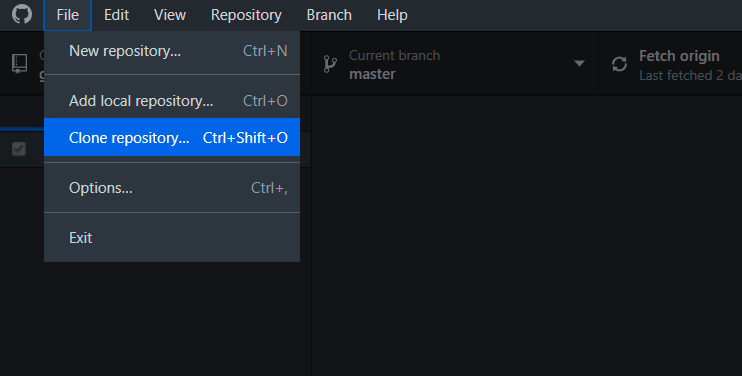
\includegraphics[width=0.5\linewidth]{figures/clonerepo.png}\hfill\strut
	\begin{itemize}
			\item Then sync (the button may say pull, fetch, or push, depending on what is to be synced):
	\end{itemize}
	\hfill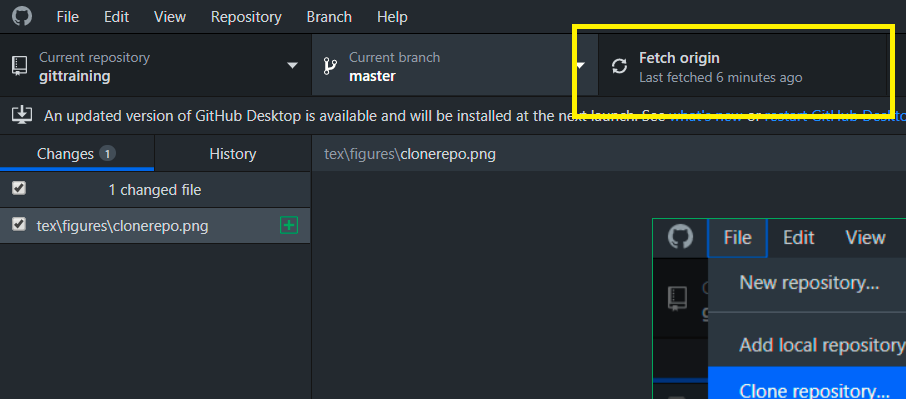
\includegraphics[width=0.5\linewidth]{figures/fetch.png}\hfill\strut
	\begin{itemize}
			\item You're ready to go!
	\end{itemize}
\end{frame}

\begin{frame}
	\frametitle{Git workflow; getting other people's edits}
	The workflow to get other people's changes is straightforward:
	\begin{enumerate}
		\item<2-> Fetch changes: this tells git to check if there's any changes on the server.
		\item<2-> Pull changes: if there are changes, this tells git to download them
	\end{enumerate}
	\only<3>{I will now create a file called example.do which we will all edit later on. Take the above steps to download it.}
\end{frame}

%------------------------------------------------
\subsection{Syncing your own changes}
%------------------------------------------------


\begin{frame}
	\frametitle{Git workflow: making edits}
	\only<1>{The general workflow to get your changes onto the git server is:}
	\only<2>{Expanding on this:}
	\only<3,4>{So forget about staging!}
	\only<5>{All things together:}
	\begin{enumerate}
  		\item<1-> Change or add File
  		\only<1-2>{\item \textbf{Stage} changed file} \only<3->{\item \textcolor{gray}{\textbf{Stage} changed file}}
  		\only<2>{
  			\begin{itemize}
	  			\item This tells Git that you've changed the file. 
	  			\item GitHub Desktop does this automatically!
  			\end{itemize}
  		}
	  	\item<1-> \textbf{Commit} change
		\only<3,5>{
			\begin{itemize}
				\item This adds the changes you've staged to your \textbf{local} repository.
				\item Git now saves a snapshot of the state of your project.
				\item This means you can undo all the changes you've made since the last commit.
			\end{itemize}
		}
	  	\item<1-> \textbf{Push} Commit(s)
	   	\only<4,5>{
	   		\begin{itemize}
	  			\item Commits will be uploaded to the remote repository (the github server for now).
				\item Others can now \textbf{Pull} your changes
				\item Your repo must be up-to-date if you're going to Push (else you may push outdated things!), so you may have to pull first (git will tell you)
	  		\end{itemize}
	  	}
	\end{enumerate}
\end{frame}


\begin{frame}
	\frametitle{Now you!}
	One by one:
	\begin{enumerate}
		\item Add a file to the folder where you've put your repository. For example: Koen.txt
		\item Commit the change (press "Commit to Master" in bottom left). GitHub Desktop may prefill a summary for you. 
		  	These are always in present tense, as it describes what is done when the commit is applied.
		\item Push the change to the central repository: Repository - Push
		\item If you try to push at the same time, you may get an error, just try again later. 
		\item If the repo has been changed before you try to push, you need to pull first:  Repository - Pull 
	\end{enumerate}
\end{frame}

\begin{frame}
	\frametitle{Notes:}
	\begin{enumerate}
		\item It all works fairly similar to Dropbox, but you have to do things manually. This may or may not be a good thing.
		\item To prevent having to pull other people's work everytime you want to push, you can make sure to work in your own branch (more on that later).
		\item You can do all we've done from the command line, but it'd be more trouble than it's worth.
		\item In the "History" tab of GitHub Desktop you can see all the commits. You can right-click any commit to revert it. 
		\item Reverting creates a new commit, which you can then revert as well!
	\end{enumerate}
\end{frame}

%------------------------------------------------
\subsection{Dealing with other people}
%------------------------------------------------

\begin{frame}
	\frametitle{Resolving Conflicts}
	Editing one file without conflicts:
	\begin{enumerate}
		\item<2-> In the file example.do, everyone add something to their own line, and commit your changes;
		\item<2-> Then we'll have to sync it all by pulling and then pushing;
		\item<2-> At the end of all this, we'll have one file that everyone edited, simultaneously.
	\end{enumerate}
	A conflict does occur if you try to pull a commit that edits a line that you've already commited changes to in your own local repo. Let's try to create conflicts:
	\begin{enumerate}
		\item<3-> Now, two people your name to the line saying "Add your name here:", commit, and sync changes.
		\item<3-> One person must now resolve the conflict. Open the file with the conflict, and make the edits necessary:
	\end{enumerate}
	
\end{frame}

\begin{frame}
	This is how git tags a conflict within the file:
	\hfill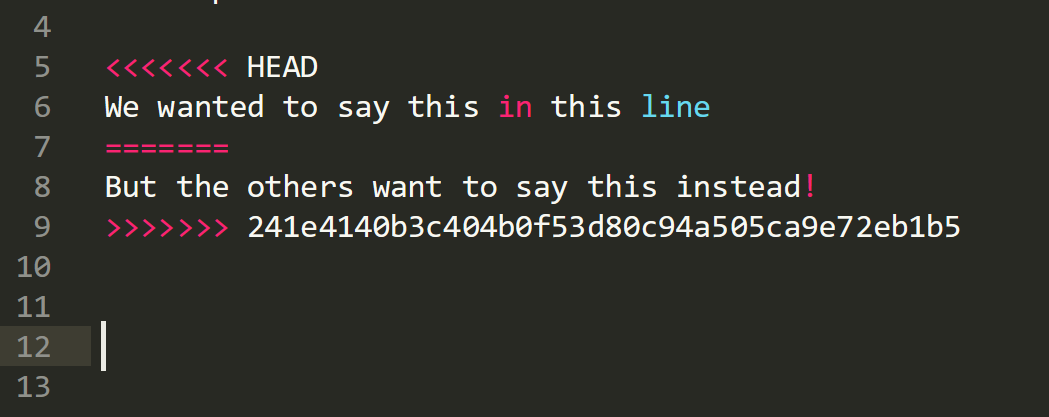
\includegraphics[width=1\linewidth]{figures/conflict.png}\hfill\strut
	Notes:
	\begin{enumerate}
		\item HEAD is us. To be precise, it's the most recent version of files that we have.
		\item The long string of letters and numbers is the SHA of the commit that is conflicting with our work. Each commit has a unique SHA.
	\end{enumerate}
\end{frame}


\begin{frame}
	\frametitle{Branches}
	\begin{itemize}
		\item \textbf{Branches} allow you to have your multiple versions of all the files in the repo, at the same time;
		\item You can edit things in your branch, while leaving the main branch (\textbf{MASTER}) untouched.
		\item Of course, this means that you are also not bothered by other people's changes!
		\item Once you're happy with the changes you've made and feel they're ready to be shared, you can \textbf{merge} your branch back into master.
		\item Merging works like pulling all changes in one go: meaning you'll have to resolve conflicts.
	\end{itemize}
\end{frame}


\begin{frame}
	\frametitle{Branches}
	Now:
	\begin{itemize}
		\item Create a branch.
		\item Make items to whatever you want
		\item Commit these changes to your own branch.
		\item Keep your branch synced with the remote as you wish.
		\item At the end, merge your branch back into the MASTER branch.
\end{frame}

%------------------------------------------------
\section{Final thoughts}
%------------------------------------------------

\begin{frame}
	\frametitle{Final thoughts}
	\begin{itemize}
		\item Today was complicated because we were all editing a bunch of files. Normally, you'd only edit a few files with a few people.
		\item Your collobarators (DPs) technically don't need to use git for it to be useful. Just make a branch where you keep their changes, and a branch where you keep yours and merge this from time to time, and share the results back to the collaborator.
		\item Explore the github website to find all versions of all files. Note how much information there is to process, not quite user-friendly!
	\end{itemize}
\end{frame}



% %------------------------------------------------

% \begin{frame}
% \frametitle{Blocks of Highlighted Text}
% \begin{block}{Block 1}
% Lorem ipsum dolor sit amet, consectetur adipiscing elit. Integer lectus nisl, ultricies in feugiat rutrum, porttitor sit amet augue. Aliquam ut tortor mauris. Sed volutpat ante purus, quis accumsan dolor.
% \end{block}

% \begin{block}{Block 2}
% Pellentesque sed tellus purus. Class aptent taciti sociosqu ad litora torquent per conubia nostra, per inceptos himenaeos. Vestibulum quis magna at risus dictum tempor eu vitae velit.
% \end{block}

% \begin{block}{Block 3}
% Suspendisse tincidunt sagittis gravida. Curabitur condimentum, enim sed venenatis rutrum, ipsum neque consectetur orci, sed blandit justo nisi ac lacus.
% \end{block}
% \end{frame}

% %------------------------------------------------

% \begin{frame}
% \frametitle{Multiple Columns}
% \begin{columns}[c] % The "c" option specifies centered vertical alignment while the "t" option is used for top vertical alignment

% \column{.45\textwidth} % Left column and width
% \textbf{Heading}
% \begin{enumerate}
% \item Statement
% \item Explanation
% \item Example
% \end{enumerate}

% \column{.5\textwidth} % Right column and width
% Lorem ipsum dolor sit amet, consectetur adipiscing elit. Integer lectus nisl, ultricies in feugiat rutrum, porttitor sit amet augue. Aliquam ut tortor mauris. Sed volutpat ante purus, quis accumsan dolor.

% \end{columns}
% \end{frame}

% %------------------------------------------------
% \section{Second Section}
% %------------------------------------------------

% \begin{frame}
% \frametitle{Table}
% \begin{table}
% \begin{tabular}{l l l}
% \toprule
% \textbf{Treatments} & \textbf{Response 1} & \textbf{Response 2}\\
% \midrule
% Treatment 1 & 0.0003262 & 0.562 \\
% Treatment 2 & 0.0015681 & 0.910 \\
% Treatment 3 & 0.0009271 & 0.296 \\
% \bottomrule
% \end{tabular}
% \caption{Table caption}
% \end{table}
% \end{frame}

% %------------------------------------------------

% \begin{frame}
% \frametitle{Theorem}
% \begin{theorem}[Mass--energy equivalence]
% $E = mc^2$
% \end{theorem}
% \end{frame}

% %------------------------------------------------

% \begin{frame}[fragile] % Need to use the fragile option when verbatim is used in the slide
% \frametitle{Verbatim}
% \begin{example}[Theorem Slide Code]
% \begin{verbatim}
% \begin{frame}
% \frametitle{Theorem}
% \begin{theorem}[Mass--energy equivalence]
% $E = mc^2$
% \end{theorem}
% \end{frame}\end{verbatim}
% \end{example}
% \end{frame}

% %------------------------------------------------

% \begin{frame}
% \frametitle{Figure}
% Uncomment the code on this slide to include your own image from the same directory as the template .TeX file.
% %\begin{figure}
% %\includegraphics[width=0.8\linewidth]{test}
% %\end{figure}
% \end{frame}

% %------------------------------------------------

% \begin{frame}[fragile] % Need to use the fragile option when verbatim is used in the slide
% \frametitle{Citation}
% An example of the \verb|\cite| command to cite within the presentation:\\~

% This statement requires citation \cite{p1}.
% \end{frame}

% %------------------------------------------------

% \begin{frame}
% \frametitle{References}
% \footnotesize{
% \begin{thebibliography}{99} % Beamer does not support BibTeX so references must be inserted manually as below
% \bibitem[Smith, 2012]{p1} John Smith (2012)
% \newblock Title of the publication
% \newblock \emph{Journal Name} 12(3), 45 -- 678.
% \end{thebibliography}
% }
% \end{frame}

% %------------------------------------------------

% \begin{frame}
% \Huge{\centerline{The End}}
% \end{frame}

% %----------------------------------------------------------------------------------------

\end{document} 